\section{Evaluation}\label{sec:eval}

\begin{figure}
  \centering
  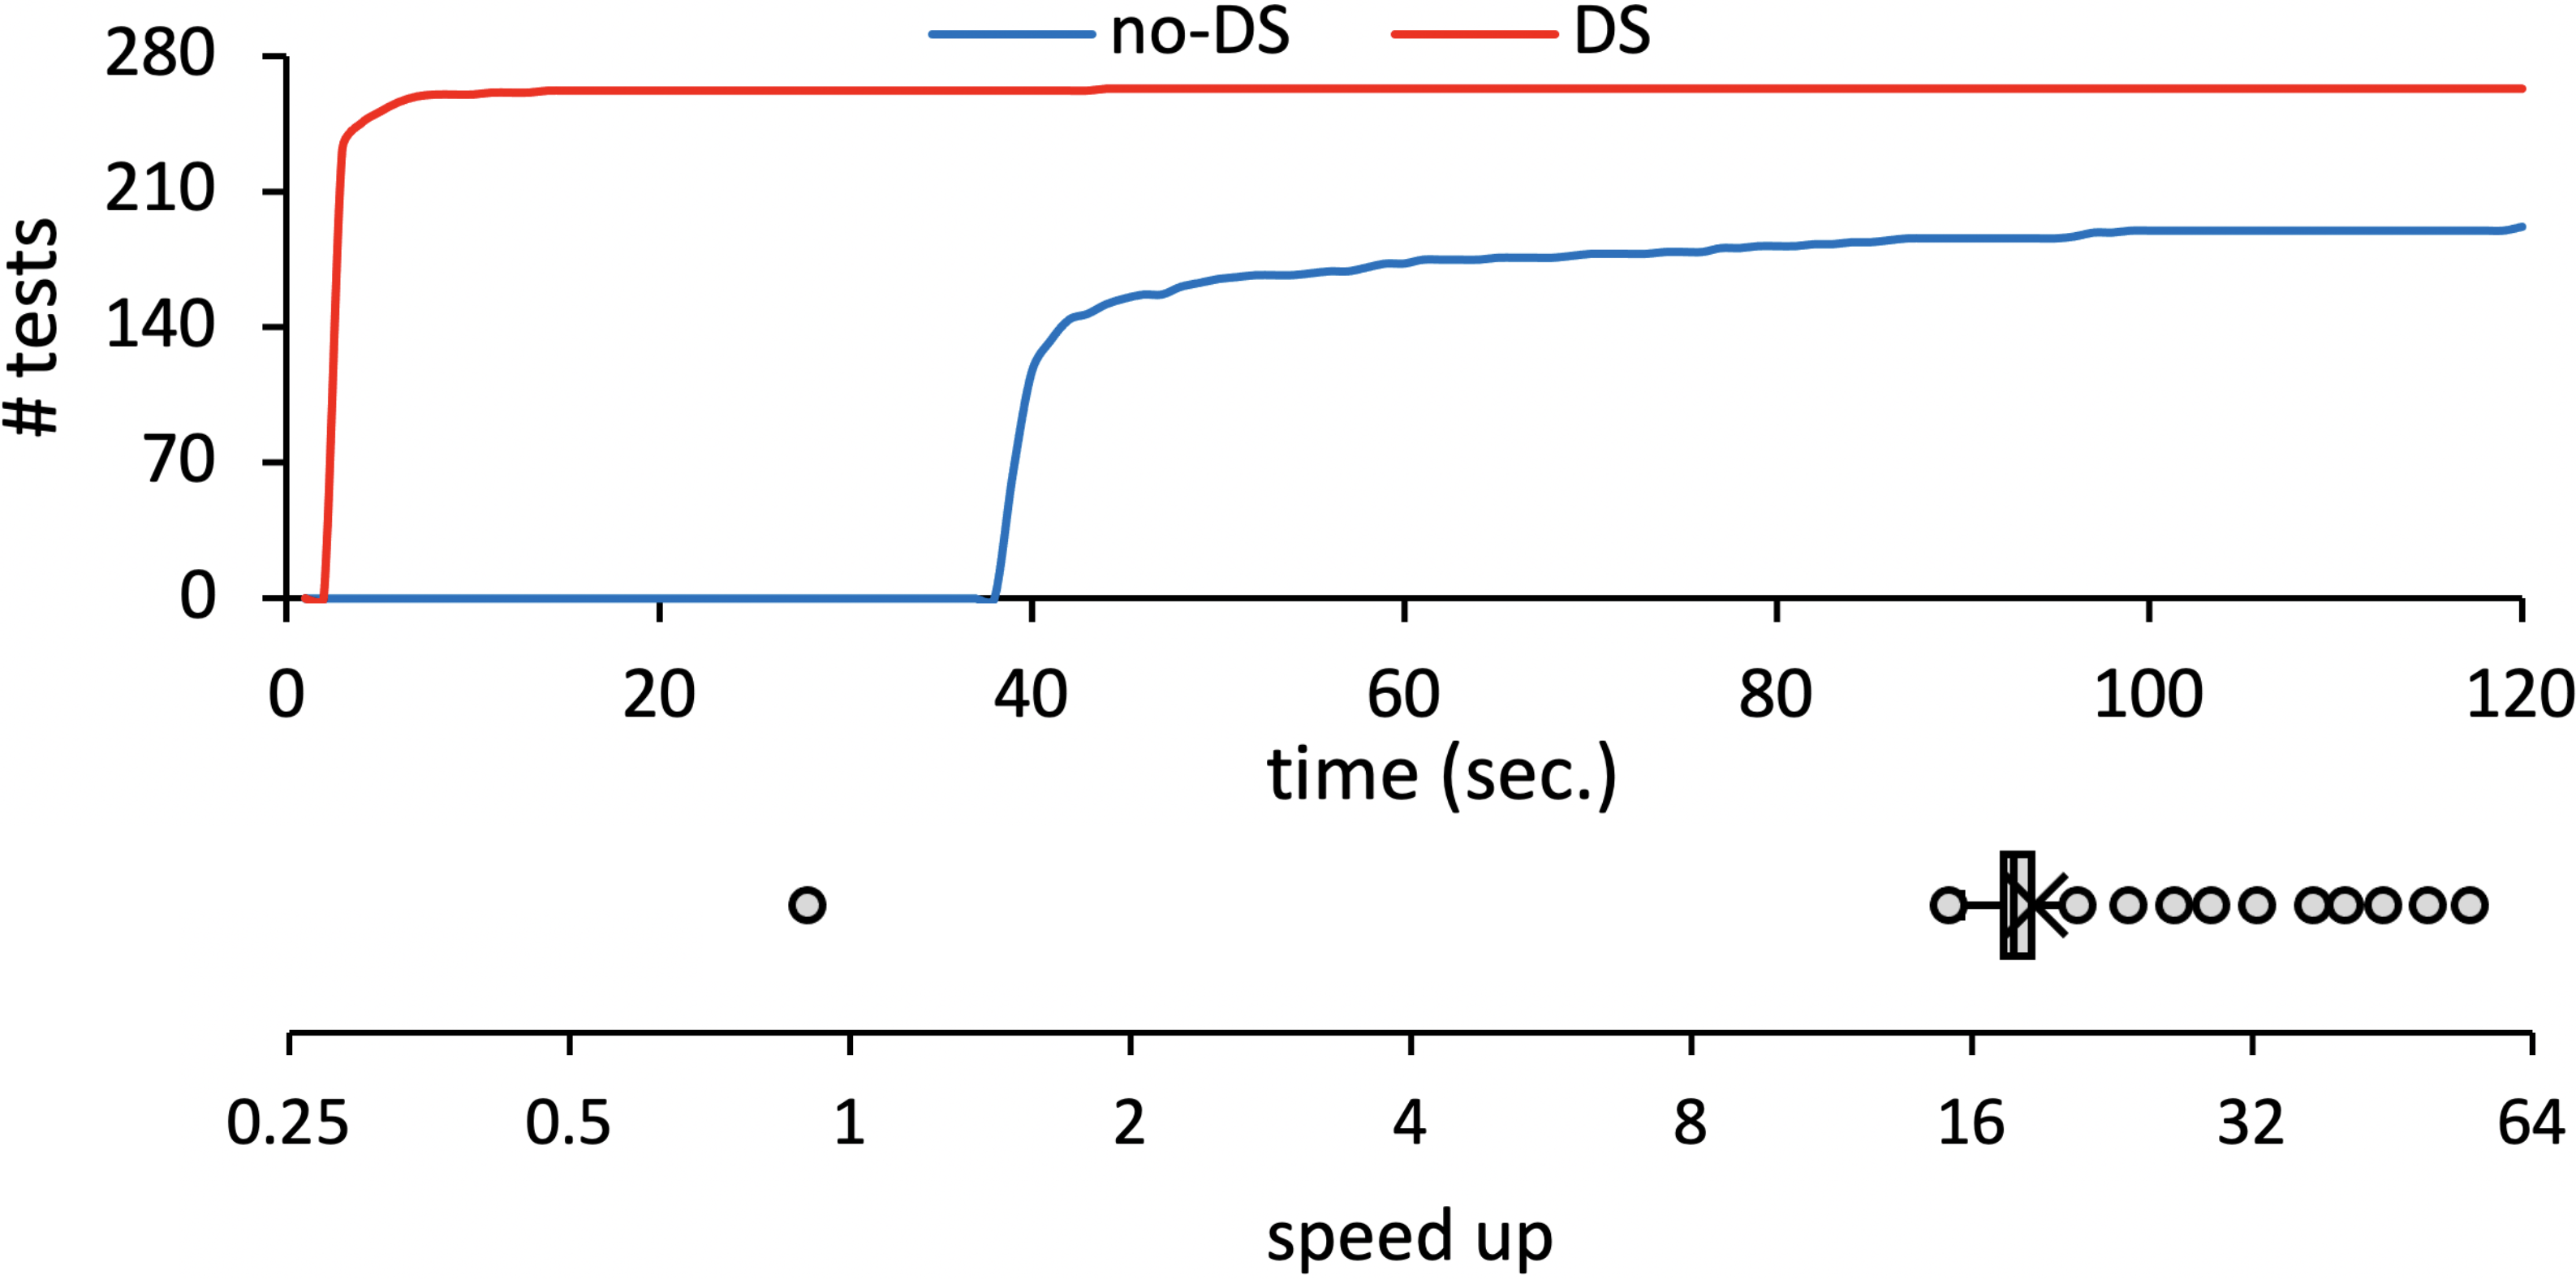
\includegraphics[width=\linewidth]{img/conc-analysis-time}
  \vspace*{-1.5em}
  \caption{Analysis time for Lodash 4 \textit{original} tests without (no-DS)
  and with (DS) dynamic shortcuts within 5 minutes}
  \label{fig:conc-analysis-time}
  \vspace*{-1.5em}
\end{figure}

We evaluated our tool based on the following three research questions:
\begin{itemize}
\item \textbf{RQ1) Analysis Speed-up:} How much analysis time is reduced by
using dynamic shortcuts during static analysis?
\item \textbf{RQ2) Precision Improvement:} How much analysis precision is
improved by using dynamic shortcuts instead of manual modeling?
\item \textbf{RQ3) Opaque Function Coverage:} How many opaque functions are
covered by dynamic shortcuts without using manual modeling?
\end{itemize}
We selected the official 306 tests of Lodash 4
(v.4.17.20)\footnote{https://github.com/lodash/lodash/blob/4.17.20/test/test.js}
used in the motivating examples in Section~\ref{sec:motivation} as our evaluation target.
The most recent papers about JavaScript static analysis techniques~\cite{value-refinement,
value-partitioning} also used the tests to evaluate their techniques.
Among them, we filtered out 37 tests that use JavaScript language
features SAFE does not support such as dynamic code generation using
\jscode{Function}, getters and setters, and browser-specific features like $\jscode{__proto__}$.
Thus, we used 269 out of 306 tests for the evaluation of $\tool$.
We performed our experiments on a Ubuntu machine
equipped with 4.2GHz Quad-Core Intel Core i7 and 64GB of RAM.


\subsection{Analysis Speed-up}

\begin{figure}[t]
  \centering
  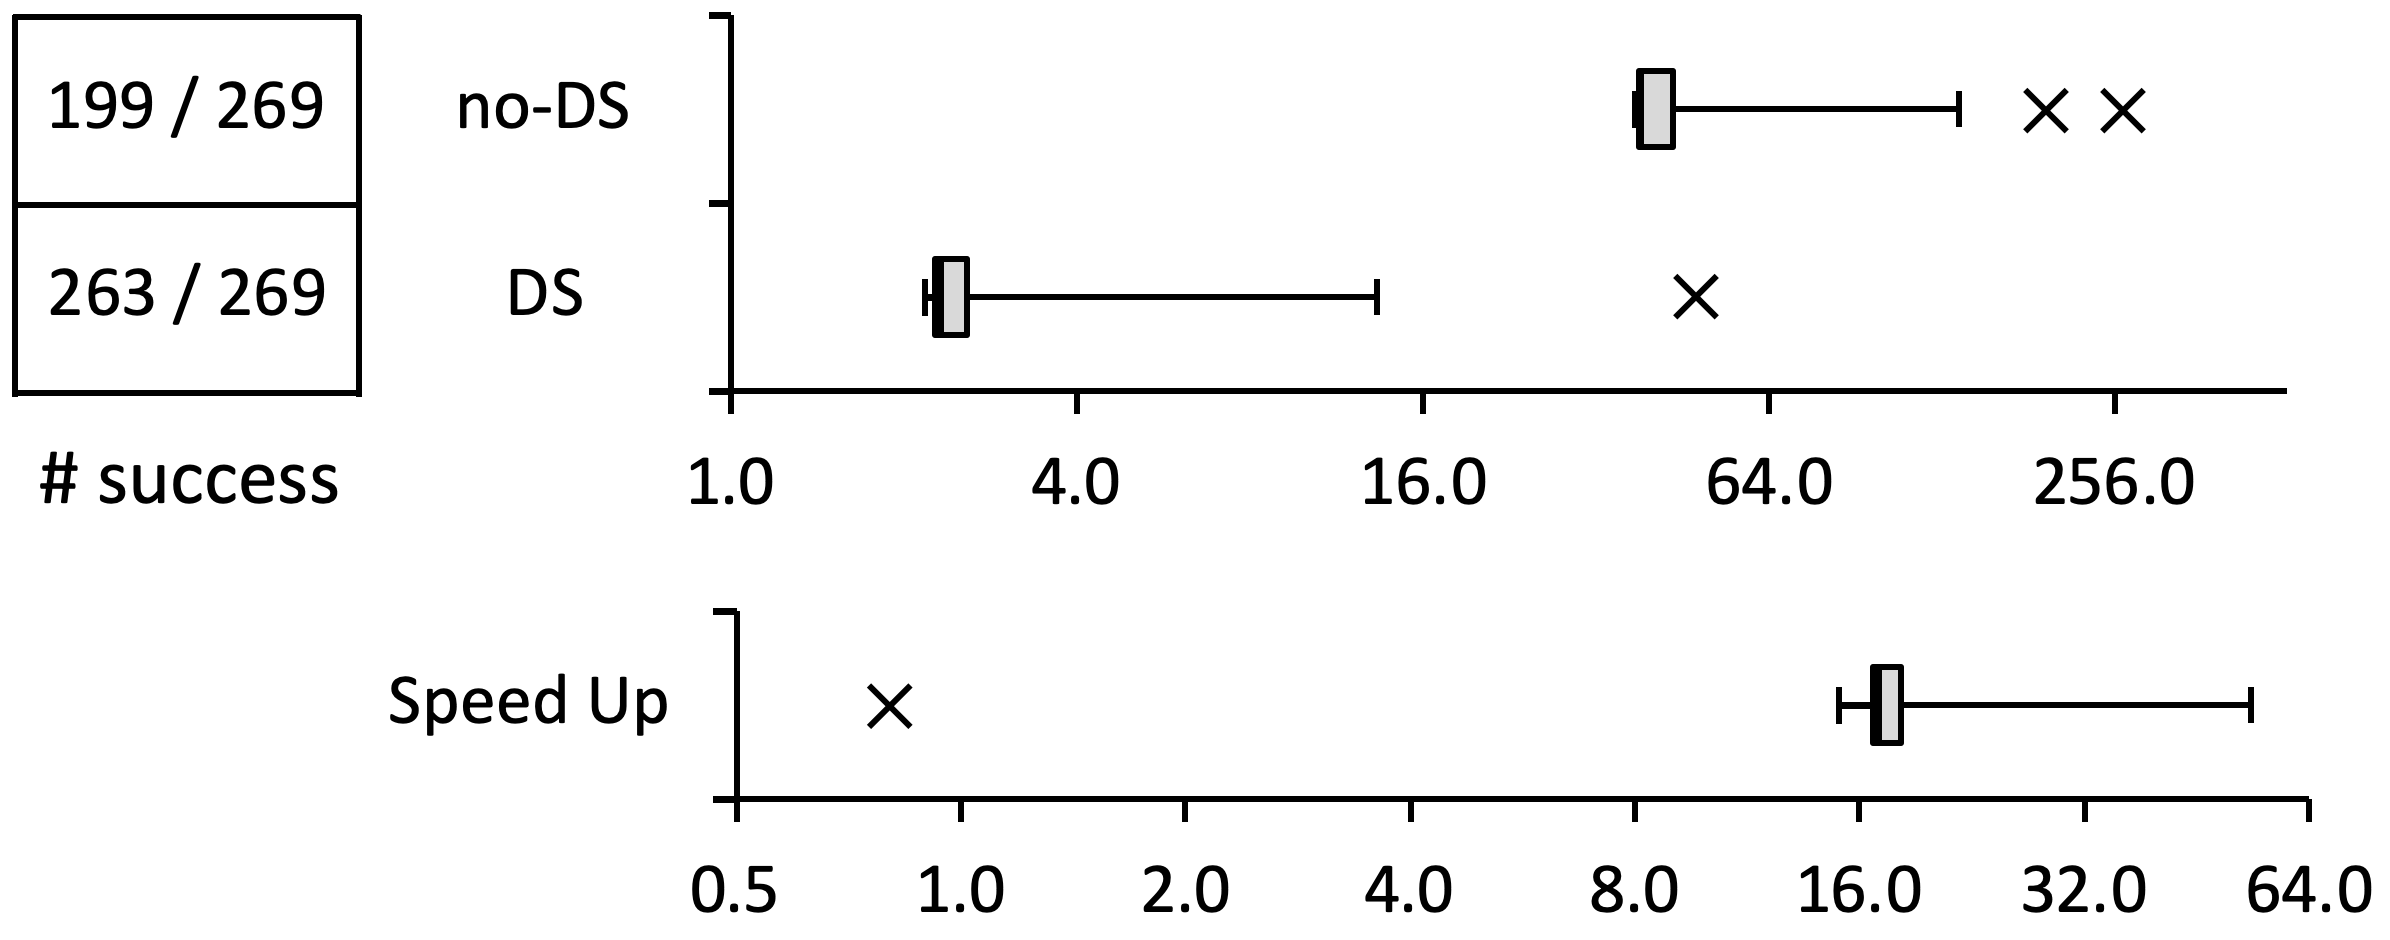
\includegraphics[width=\linewidth]{img/abs-analysis-time}
  \vspace*{-1.5em}
  \caption{Analysis time for Lodash 4 \textit{abstracted} tests without (no-DS)
  and with (DS) dynamic shortcuts within 5 minutes}
  \label{fig:abs-analysis-time}
  \vspace*{-1.5em}
\end{figure}

To evaluate the effectiveness of using dynamic shortcuts, we performed static
analysis of 269 Lodash 4 tests with and without dynamic shortcuts.
Figure~\ref{fig:conc-analysis-time} depicts cumulative distribution charts for
their analysis time and a box plot in a logarithmic scale for speed up after
applying dynamic shortcuts.  In the upper chart, the $x$-axis is time and the
$y$-axis shows the number of tests until the time.  While the baseline analysis
(no-DS) finished analysis of 200 out of 269 tests within 5 minutes, our tool
(DS) finished analysis of 263 tests using dynamic shortcuts.  For finished
tests, the average analysis time is 49.57 seconds for no-DS and 2.78 seconds for
DS.  Since only few tests analyzed in 2 to 5 minutes (8 tests for no-DS
and no tests for DS), we only show the results until 2 minutes on the
cumulative distribution charts to show the difference between their results more
clearly.  Among 200 tests analyzed by no-DS, two tests are timeout in DS thus
198 tests are analyzable by both analyzers. For them, we depicts the box plot for
analysis speed up by applying dynamic shortcuts.  It shows that tsing dynamic
shortcuts outperforms the baseline analyzer at most 54.98$\x$ and 19.96$\x$ on
average.  Only for one test using $\jscode{_.sample}$, a Lodash 4 library
function that randomly samples a value from a given array, DS showed
0.90$\x$ speed of no-DS due to frequent use of dynamic shortcuts, that is 24
times.

Note that since most Lodash 4 tests use concrete values instead of
non-deterministic user inputs, they can be analyzed by a few number of dynamic shortcuts.
In fact, among 269 tests, 262 tests are analyzed
by a single dynamic shortcut without using abstract semantics.
However, in real-world JavaScript programs, arguments of library
functions may include non-deterministic user inputs.
To evaluate our approach in a real-world setting,
we modified Lodash 4 official tests with abstract values to simulate actual use patterns of library functions.
We mad abstract values by randomly selecting literals and replacing
one of them with its corresponding abstract value.
For example, if we select a numeric literal \jscode{42}, we modified it to the abstract numeric value
$\top_{\code{num}}$, which represents all the numeric values.
In the remaining section, we evaluated $\tool$ using the \textit{original} tests
and the \textit{abstracted} tests of Lodash 4.

For abstracted tests as well, dynamic shortcuts successfully accelerated the static analysis.
Figure~\ref{fig:abs-analysis-time} shows the analysis time of the abstracted tests.
Only 4 tests for no-DS and 9 tests for DS are finished between 2 to 5 minutes.
Among 269 abstracted tests, no-DS finished analysis of 158 tests within 5 minutes,
but DS finished analysis of 168 tests.  For finished tests, the average analysis
time is 44.88 seconds for no-DS and 42.28 seconds for DS. Among 158 tests analyzed by no-DS, DS
fails to analysis 15 tests in the time limit thus 143 tests are analyzable by
both analyzers.  For them, the dynamic shortcuts outperforms the baseline
analyzer at most 50.60$\x$ and 6.30$\x$ on average.

\begin{figure}[t]
  \centering
  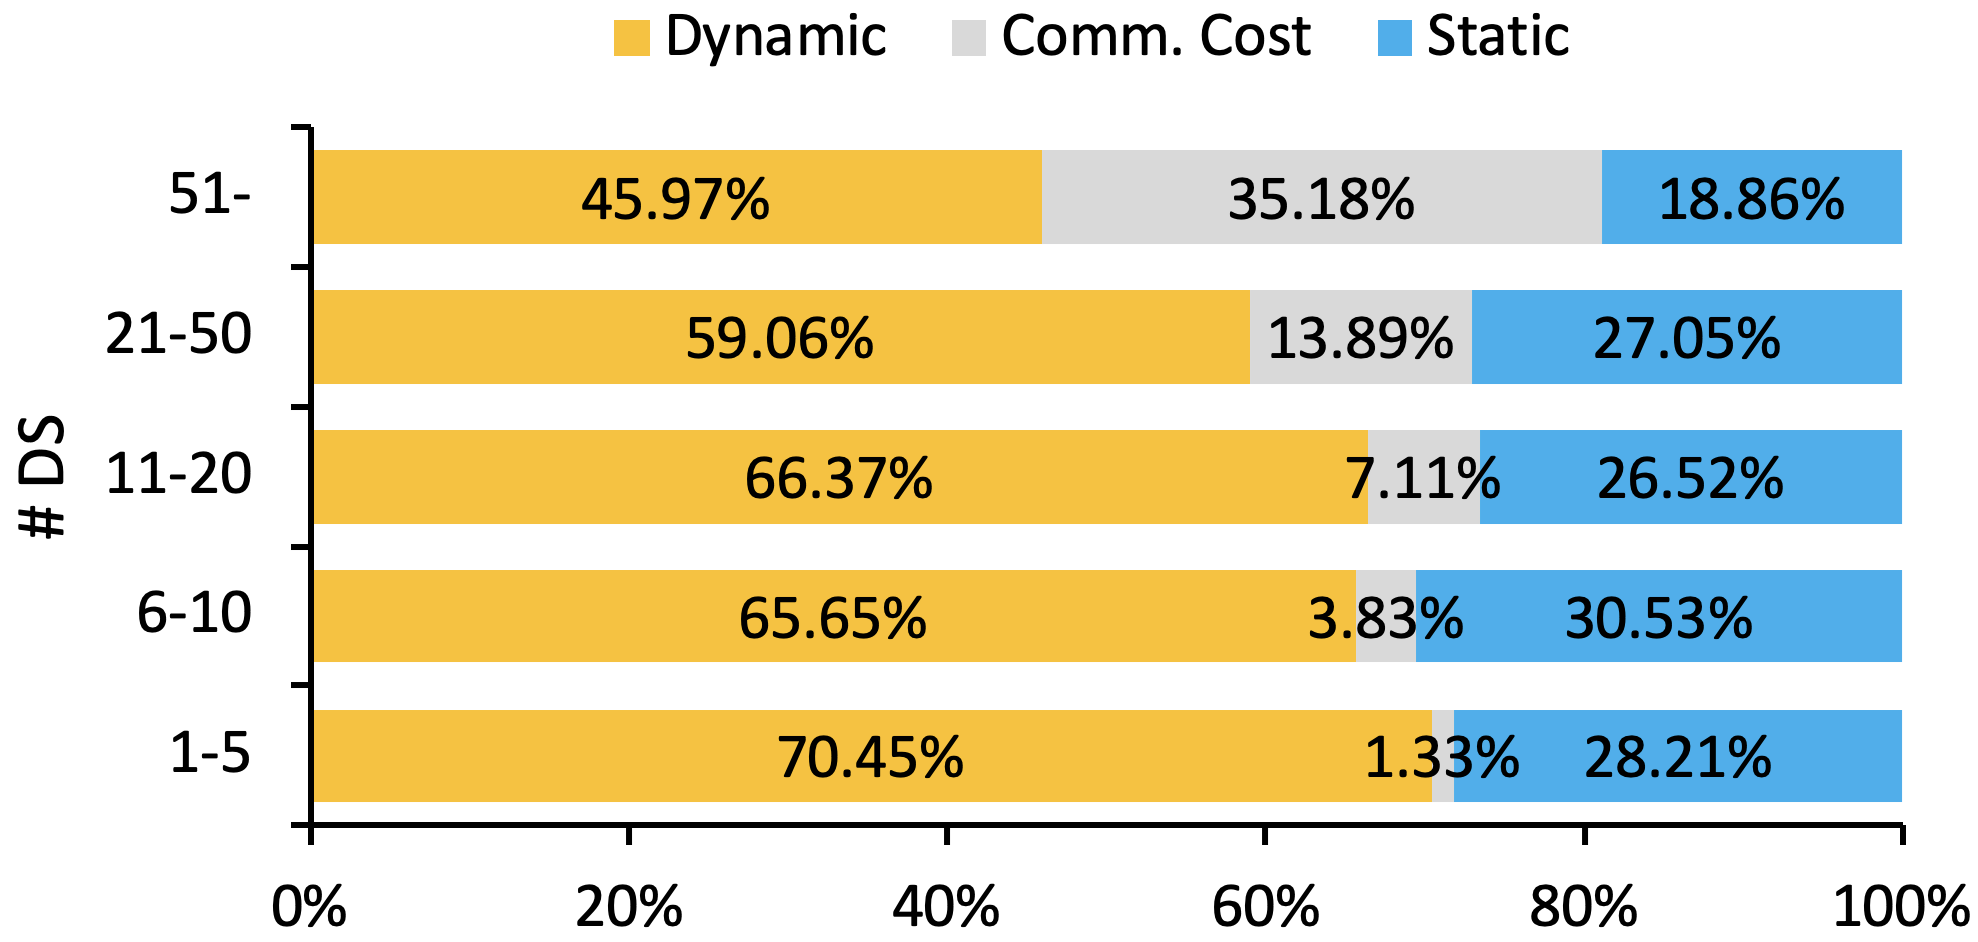
\includegraphics[width=\linewidth]{img/abs-analysis-ratio}
  \vspace*{-1.5em}
  \caption{Analysis time ratio for 143 \textit{abstracted} tests}
  \label{fig:abs-analysis-ratio}
  \vspace*{-1.5em}
\end{figure}

\begin{table*}[t]
  \centering
  \caption{The number of \textit{abstracted} tests using dynamic shortcut
  instead of manual modeling for each JavaScript built-in library}
  \label{table:func-replace}
  \vspace*{-1em}
  \scriptsize
  \[
    \begin{array}{c|l|c|c?c|l|c|c?c|l|c|c}

      \myhead{Object}       {Function}        {\# Replaced}

      \mysutf{1}{}          {Array    }  {203 / 203}{ 90 / 116} & \mysutf{1}{}             {String     }  { 20 /  20}{  9 /  10} & \mysutf{1}{}       {Object        }  {263 / 263}{151 / 167} \mylinefff
      \mysutf{1}{}          {new Array}  {  0 /   0}{  0 /  10} & \mysutf{1}{}             {toString   }  {  0 /   0}{  0 /  33} & \mysutf{1}{}       {new Object    }  {  0 /   0}{  0 /   3} \mylinefff
      \mysutf{1}{}          {isArray  }  {263 / 263}{144 / 167} & \mysutf{1}{}             {valueOf    }  {  0 /   0}{  0 /  12} & \mysutf{1}{}       {getPrototypeOf}  { 56 /  56}{ 24 /  29} \mylinefff
      \mysutf{1}{}          {concat   }  {263 / 263}{163 / 167} & \mysutt{1}{}             {charAt     }  {  7 /   7}{  5 /   5} & \mysutf{1}{}       {create        }  {263 / 263}{164 / 167} \mylinefff
      \mysutf{1}{}          {join     }  {263 / 263}{166 / 167} & \mysutf{1}{}             {charCodeAt }  { 15 /  15}{  3 /   4} & \mysutf{1}{Object} {defineProperty}  {263 / 263}{160 / 167} \mylinefff
      \mysutf{1}{}          {pop      }  { 25 /  25}{  9 /  13} & \mysutt{1}{}             {indexOf    }  {  2 /   2}{  1 /   1} & \mysbtt{1}{}       {freeze        }  {  1 /   1}{  1 /   1} \mylinefff
      \mysutf{2}{Array}     {push     }  {263 / 263}{150 / 167} & \mysutf{1}{String}       {match      }  { 25 /  25}{ 11 /  13} & \mysutf{1}{}       {keys          }  {263 / 263}{161 / 167} \mylinefff
      \mysutt{1}{}          {reverse  }  { 10 /  10}{  3 /   3} & \mysutf{1}{}             {replace    }  { 55 /  55}{ 19 /  26} & \mysutf{1}{}       {toString      }  {263 / 263}{129 / 167} \mylinefff
      \mysutf{1}{}          {shift    }  {  2 /   2}{  0 /   1} & \mysutf{1}{}             {slice      }  {263 / 263}{165 / 167} & \mysutf{1}{}       {hasOwnProperty}  {263 / 263}{161 / 167} \mylinefft
      \mysutf{1}{}          {slice    }  {263 / 263}{164 / 167} & \mysutf{1}{}             {split      }  {  5 /   5}{  0 /   1} & \mysutf{1}{}       {parseInt}        {  1 /   1}{  0 /   1} \mylinefff
      \mysutf{1}{}          {sort     }  { 69 /  69}{ 26 /  28} & \mysutf{1}{}             {substring  }  {214 / 214}{ 91 / 121} & \mysutf{1}{Global} {isNaN   }        { 15 /  15}{  9 /  25} \mylinefff
      \mysutf{1}{}          {splice   }  { 25 /  25}{  6 /  11} & \mysutf{1}{}             {toLowerCase}  {214 / 214}{ 90 / 121} & \mysbtt{1}{}       {isFinite}        {  3 /   3}{  1 /   1} \mylinefft
      \mysutt{1}{}          {unshift  }  {  2 /   2}{  1 /   1} & \mysutf{1}{}             {toUpperCase}  { 10 /  10}{  4 /   6} & \mysbtt{1}{}       {RegExp    }      {263 / 263}{167 / 167} \mylineftf
      \mysutf{1}{}          {indexOf  }  { 94 /  94}{ 22 /  47} & \mysutt{2}{Boolean}      {Boolean}      {  3 /   3}{  2 /   2} & \mysutf{2}{RegExp} {new RegExp}      {  0 /   0}{  0 /   1} \mylinefff
      \mysutf{1}{}          {every    }  { 92 /  92}{ 23 /  32} & \mysutf{1}{}             {valueOf}      {  0 /   0}{  0 /   6} & \mysbtt{1}{}       {exec      }      {263 / 263}{167 / 167} \mylinettf
      \mysutt{1}{}          {ceil }      { 36 /  36}{  8 /   8} & \mysutf{2}{Number}       {Number }      {  2 /   2}{  1 /   2} & \mysutf{1}{}       {test      }      {263 / 263}{158 / 167} \mylinefft
      \mysuff{1}{}          {floor}      { 16 /  17}{  4 /   5} & \mysutf{1}{}             {valueOf}      {  0 /   0}{  0 /  16} & \mysutf{1}{}       {Error         }  {  1 /   1}{  0 /   1} \mylineftf
      \mysutf{1}{Math}      {max  }      {263 / 263}{134 / 167} & \mysutt{1}{}             {toString}     {263 / 263}{167 / 167} & \mysutf{2}{Error}  {new Error     }  {  0 /   0}{  0 /   8} \mylinefff
      \mysutf{1}{}          {min  }      { 64 /  64}{ 15 /  48} & \mysutf{1}{Function}     {apply   }     {263 / 263}{124 / 167} & \mysutf{1}{}       {new RangeError}  {  0 /   0}{  0 /   3} \mylinefff
      \mysutt{1}{}          {pow  }      { 11 /  11}{  5 /   5} & \mysuff{1}{}             {call    }     {262 / 263}{ 50 / 167} & \mysutf{1}{}       {new TypeError }  {  0 /   0}{  0 /   9}
    \end{array}
  \]
  \vspace*{-1em}
\end{table*}

Unlike for the original tests, analysis of 143
abstracted tests that are analyzable by both analyzers invoked
16.05 dynamic shortcuts.  Because taking a dynamic shortcut
requires converting between abstract states and sealed symbolic values
and exchanging them between the static analyzer and the dynamic analyzer,
using dynamic shortcuts multiple times may incur more performance
overhead than performance benefits by using sealed symbolic execution.
One may conjecture that the communication cost between the static
analyzer and the dynamic analyzer may be proportional to the number of
dynamic shortcuts.

To experimentally evaluate the conjecture, we investigated the relationship between
the communication cost between analyzers and the number of dynamic shortcuts.
For 198 original tests, the communication cost was only
\inred{x.xx}\% of the total analysis time.  However, for 143
abstracted tests, the communication cost was 82.49\% of the
total analysis time.  Figure~\ref{fig:abs-analysis-ratio} presents the
analysis time ratio for 143 abstracted tests.
The $x$-axis represents the time ratio normalized by the total analysis time of
the baseline analysis (no-DS) and the $y$-axis denotes the number of dynamic
shortcuts and the number of corresponding tests.
For all 143 tests, the communication cost (Comm. Cost) is larger than
both the static analysis time (Static) and the dynamic analysis
time (Dynamic).  When dynamic shortcuts are performed less than 10 times,
the communication cost is modest compared with the baseline static
analysis time.  However, the more dynamic shortcuts are performed,
the less the performance benefits by using sealed symbolic execution.
Specifically, when dynamic shortcuts are performed more than
20 times, DS-Comm. is even larger than no-DS.
Based on this evaluation result, we believe that we can leverage
dynamic shortcuts by optimizing the communication between static and dynamic analyzers.

\begin{figure}[t]
  \centering
  \begin{subfigure}[t]{0.48\textwidth}
    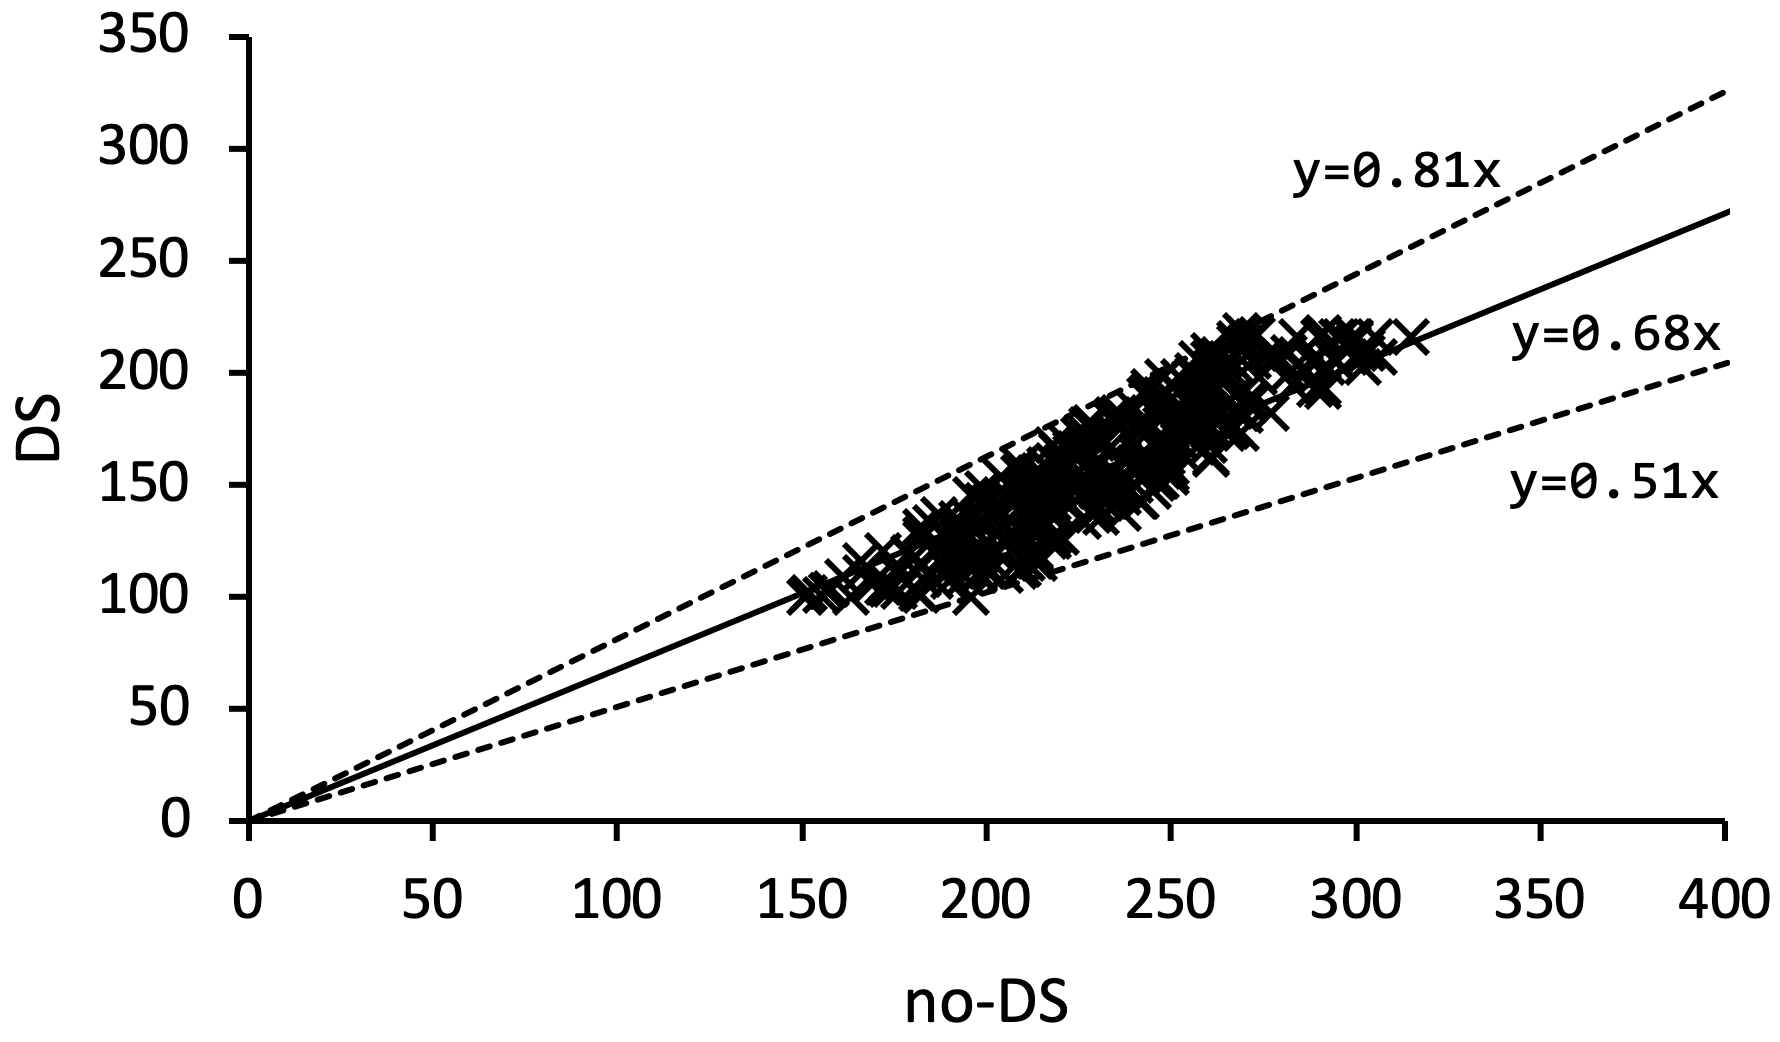
\includegraphics[width=\linewidth]{img/conc-precision}
    \vspace*{-1.5em}
    \caption{Reachable branches for 198 \textit{original} tests}
    \label{fig:precision-fail}
  \end{subfigure}
  \begin{subfigure}[t]{0.48\textwidth}
    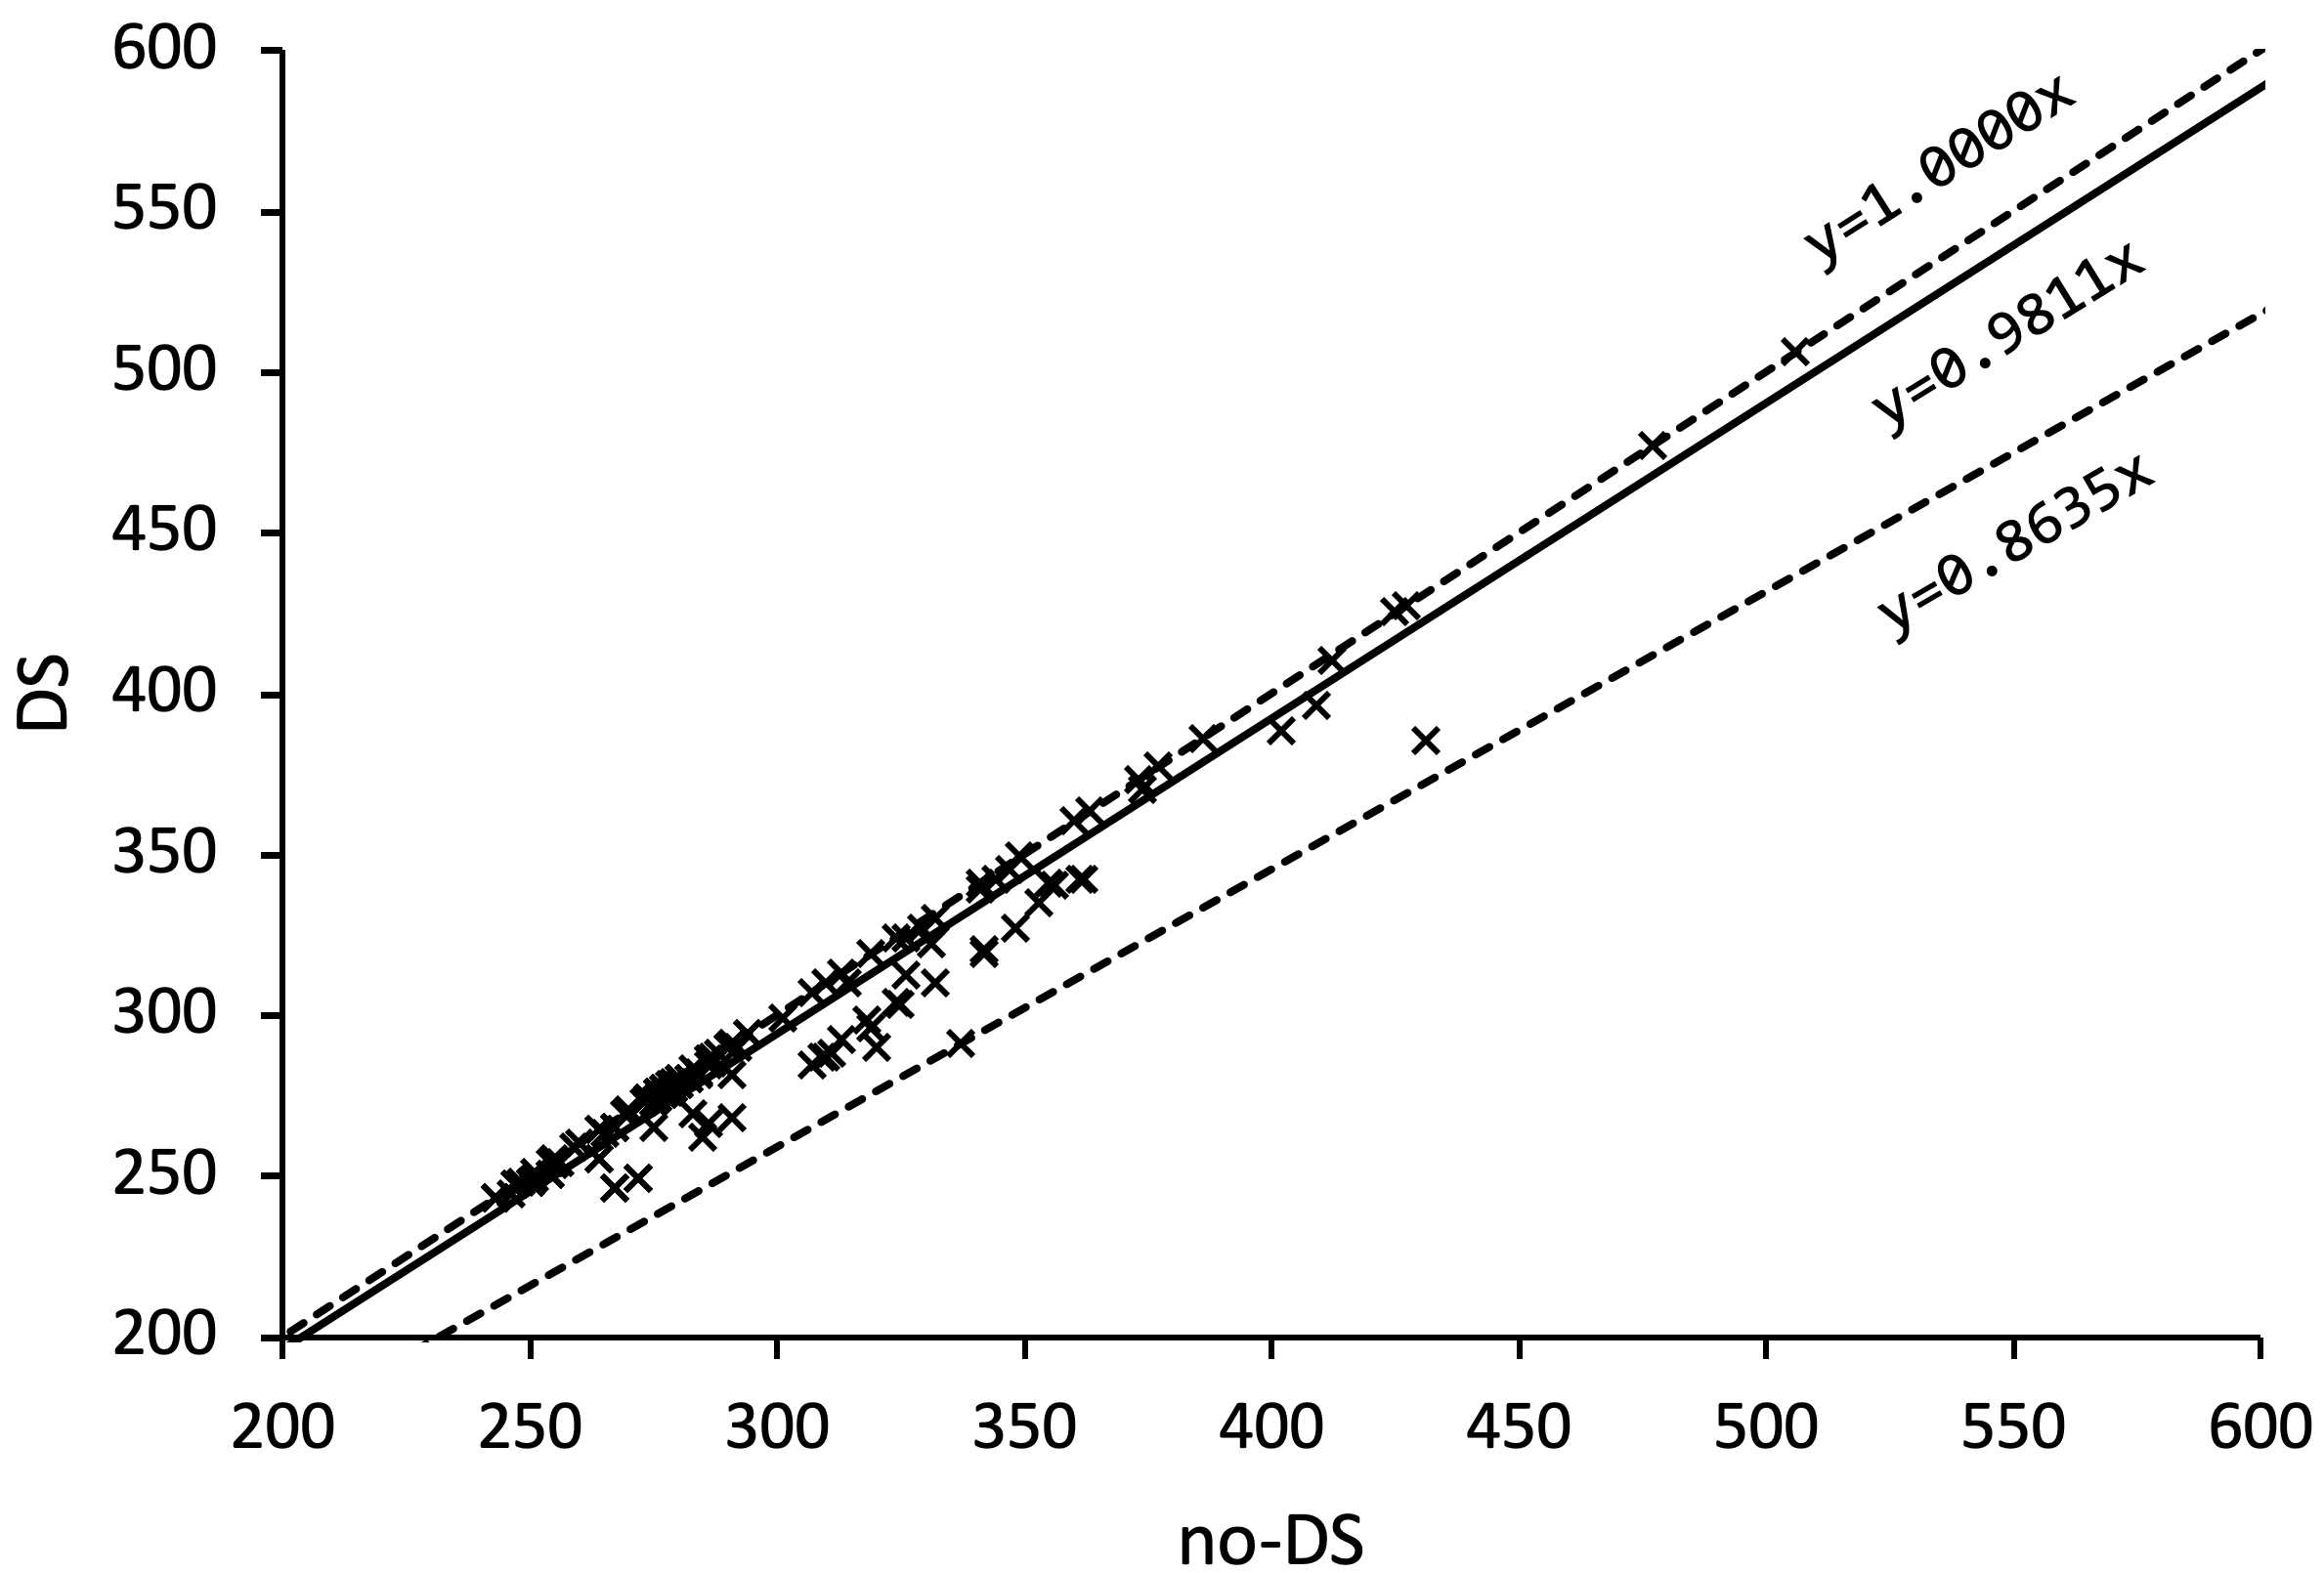
\includegraphics[width=\linewidth]{img/abs-precision}
    \vspace*{-1.5em}
    \caption{Reachable branches for 143 \textit{abstracted} tests}
    \label{fig:precision-branch}
  \end{subfigure}
  \vspace*{-1em}
  \caption{Branch coverage of analysis without (no-DS) and with (DS) dynamic shortcuts}
  \label{fig:precision}
  \vspace*{-1.5em}
\end{figure}



\subsection{Precision Improvement}

To evaluate the analysis precision improvement of dynamic shortcuts,
we measured the number of branches covered by no-DS and DS.
Because both no-DS and DS are designed to be sound,
high (low) branch coverage denotes low (high) analysis precision.

Figure~\ref{fig:precision} depicts the comparison of the analysis
precision between no-DS and DS.  The $x$-axis and the $y$-axis denote
the number of branches covered by no-DS and DS, respectively;
each $\times$ mark denotes each test.  The top and bottom dotted lines
denote the worst and the best precision improvement, respectively, and
the middle solid line denotes the average improvement.
For 198 original tests that are analyzable by both analyzers,
Figure~\ref{fig:precision}(a) shows that dynamic shortcuts
reduced the number of covered branches at most 13.13\%. However, it reduced
the number of branches 0.46\% on average because the most of original tests
use concrete values without any non-determinism. Unlike original tets, for 143
abstracted tests that are analyzable by both analyzers,
Figure~\ref{fig:precision}(b) shows that dynamic shortcuts successfully cut down
the number of covered branches at most 13.65\% and 1.89\% on average.  In other
words, the dynamic shortcuts prevent to analyze 1.44 and 5.97 spurious branches
for original and abstracted tests on average.


\subsection{Opaque Function Coverage}
To evaluate how much manual modeling efforts of opaque functions
are reduced by dynamic shortcuts, we measured the number of tests where
opaque functions that are analyzed only by dynamic analysis not by
static analysis.  Table~\ref{table:func-replace} summarizes the result.
For \inred{xx} original tests and \inred{xx} abstracted tests, we measured the
number of tests that use only dynamic shortcuts instead of manual modeling
for each JavaScript built-in library function.  For each row,
\textbf{Object} column denotes a built-in object,
\textbf{Function} a function name, and
\inred{\textbf{\# Replaced} the number of tests successfully replacing manual
modeling via dynamic shortcuts with the total number of tests using the target function.
For example, the fourth row in the left side describes that \jscode{Array.prototype.toString} is used in
\inred{139} original tests and \inred{xxx} abstracted tests.
 Among them, \inred{44} original tests \inred{xx} abstracted tests are successfully analyzed
by dynamic shortcuts instead of using the modeling of
\jscode{Array.prototype.toString}.
Moreover, several built-in functions are analyzed by only dynamic shortcuts in
all tests.  Among \inred{49} JavaScript built-in functions, \inred{xx} and
\inred{xx} functions are analyzed by only dynamic shortcut instead of manual
modeling for all original and all abstracted tests, respectively.  Each filled cell
describes fully replaceable cases in Table~\ref{table:func-replace}.
Therefore, dynamic shortcuts effectively lessen
the burden of manual modeling for JavaScript built-in functions.
}
